\section{Results and diagnostics}
\begin{table}[t]
\centering\small
\begin{tabular}{lrrrr}
\toprule
Model & DNA Acc. & DNA F1 & Protein Acc. & Protein F1 \\
\midrule
Raw candidate & $91.10 \pm 0.35$ & $91.09 \pm 0.35$ & $59.97 \pm 0.56$ & $50.63 \pm 1.67$ \\
BioBPE candidate & $90.16 \pm 0.14$ & $90.16 \pm 0.14$ & $59.05 \pm 0.33$ & $50.28 \pm 0.42$ \\
BioBPE fixed head (B1) & $88.76 \pm 0.37$ & $88.76 \pm 0.37$ & $51.14 \pm 5.36$ & $38.00 \pm 4.15$ \\
Text-only candidate & $49.84 \pm 0.57$ & $33.26 \pm 0.25$ & $29.10 \pm 0.00$ & $6.44 \pm 0.00$ \\
\bottomrule
\end{tabular}

\caption{Fixed-checkpoint test results (\%, mean $\pm$ sample SD over three seeds). F1 is macro-F1 over the fixed class set. All models use the same eligible examples.}
\label{tab:main}
\end{table}
\paragraph{Candidate scoring versus the implemented fixed head.}
The \BioBPE{} candidate model attains 90.16\% DNA accuracy and 59.05\% protein accuracy (Table~\ref{tab:main}). Relative to B1, the paired mean differences are $+1.40\pm0.42$ and $+7.91\pm5.69$ percentage points, respectively; all three seeds favor candidate scoring on both tasks. Protein macro-F1 increases by $12.28\pm4.56$ points. B1 protein accuracy varies substantially, from 45.65\% to 56.35\%. This comparison supports the current candidate configuration under the tested budget, but input format, pooling, and output-layer initialization differ, so it does not isolate a causal benefit of candidate semantics.

\paragraph{Token compression does not yield a predictive or training-time gain.}
Raw candidate scoring has higher test accuracy than \BioBPE{} on both tasks: the paired \BioBPE{} differences are $-0.93\pm0.29$ points for DNA and $-0.92\pm0.49$ points for protein, negative in all seeds. The dev DNA difference was $+0.60$ points, so that advantage does not carry to test. The pooled training-input median falls from 173 to 96 tokens, but mean training time is 41.20 minutes for raw and 41.24 minutes for \BioBPE{}. Peak allocated memory rises from 7.89 to 8.41~GiB. We therefore report compression, a larger embedding matrix, and observed cost rather than infer acceleration from token counts. We did not optimize kernels or measure a separate inference-latency benchmark.

\begin{table}[t]
\centering\scriptsize
\begin{tabular}{llrrrr}
\toprule
Model & Task & NLL (raw) & NLL (cal.) & Brier (cal.) & ECE (cal.) \\
\midrule
Raw candidate & DNA & $0.243 \pm 0.014$ & $0.222 \pm 0.010$ & $0.133 \pm 0.007$ & $0.011 \pm 0.005$ \\
BioBPE candidate & DNA & $0.314 \pm 0.011$ & $0.249 \pm 0.002$ & $0.147 \pm 0.002$ & $0.022 \pm 0.001$ \\
BioBPE fixed head (B1) & DNA & $0.300 \pm 0.012$ & $0.279 \pm 0.008$ & $0.165 \pm 0.005$ & $0.018 \pm 0.001$ \\
Text-only candidate & DNA & $0.693 \pm 0.000$ & $0.693 \pm 0.000$ & $0.500 \pm 0.000$ & $0.004 \pm 0.003$ \\
Raw candidate & Protein & $1.190 \pm 0.034$ & $1.044 \pm 0.024$ & $0.529 \pm 0.009$ & $0.054 \pm 0.011$ \\
BioBPE candidate & Protein & $1.184 \pm 0.023$ & $1.057 \pm 0.014$ & $0.539 \pm 0.004$ & $0.049 \pm 0.002$ \\
BioBPE fixed head (B1) & Protein & $1.241 \pm 0.059$ & $1.236 \pm 0.063$ & $0.619 \pm 0.037$ & $0.042 \pm 0.014$ \\
Text-only candidate & Protein & $1.630 \pm 0.001$ & $1.628 \pm 0.001$ & $0.781 \pm 0.000$ & $0.009 \pm 0.007$ \\
\bottomrule
\end{tabular}

\caption{Test probability metrics (mean $\pm$ sample SD). Calibration uses the previously fitted task/checkpoint temperature. Brier is the sum of squared class-probability errors per example; ECE uses 15 equal-width bins. Lower values are better.}
\label{tab:calibration}
\end{table}
\paragraph{Probability quality.}
Previously fitted temperatures lower mean \BioBPE{} test NLL from approximately 0.31 to 0.25 for DNA and from 1.18 to 1.06 for protein (Table~\ref{tab:calibration}). Raw candidate scoring retains lower calibrated NLL, about 0.22 and 1.04. Calibration gains therefore do not reverse the representation comparison, and NLL improvement alone does not establish perfect calibration. Brier and ECE report complementary aspects of the resulting distributions. The text-only model's low ECE despite weak classification also shows why ECE alone cannot rank overall predictive quality.

\begin{figure}[t]
\centering
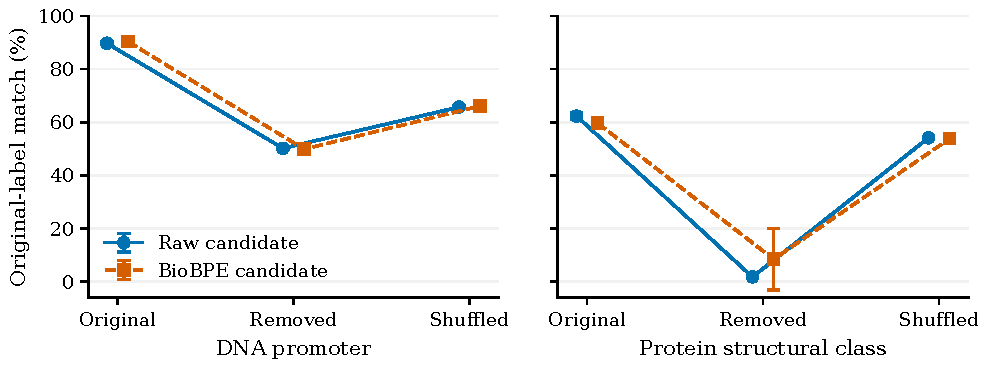
\includegraphics[width=0.91\linewidth]{figures/sequence_diagnostics.pdf}
\caption{Dev sequence-dependence diagnostics. Points and error bars are means and sample SDs across three trained seeds. For shuffled sequences, each seed first averages three deterministic character permutations. The vertical axis measures agreement with the \emph{original} labels: removed or shuffled sequences are interventions, not independently labeled biological examples.}
\label{fig:sequence}
\end{figure}
\paragraph{Sequence dependence.}
The trained text-only control reaches 49.84\% DNA and 29.10\% protein test accuracy, with a constant class prediction within each task/seed. Its low protein macro-F1 reflects the class imbalance. Dev interventions on the sequence-trained \BioBPE{} model reduce original-label matching from 90.34\% to 49.84\% after DNA removal and to 66.12\% after DNA shuffling; protein values change from 59.65\% to 8.42\% and 53.79\%, respectively (Figure~\ref{fig:sequence}). Shuffling preserves character counts but not biological labels. These observations support sequence dependence and residual composition-related signal, without identifying a learned biological mechanism. Inference-time removal is also a distribution shift and must not be equated with the separately trained text-only baseline.

\begin{figure}[t]
\centering
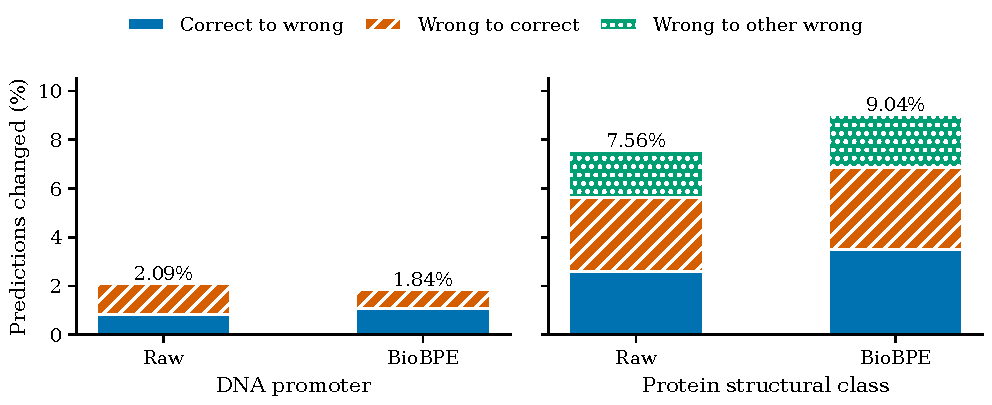
\includegraphics[width=0.91\linewidth]{figures/candidate_order.pdf}
\caption{Dev prediction changes after one deterministic nonidentity candidate permutation per example, with outputs mapped back to canonical labels. Stacks show mean fractions over three seeds. For \BioBPE{} protein predictions, correct-to-wrong and wrong-to-correct changes nearly cancel in accuracy, while wrong-to-other-wrong changes also contribute to instability.}
\label{fig:order}
\end{figure}
\paragraph{Candidate-order sensitivity.}
The same candidate set does not ensure the same prediction. On dev, reordering candidates changes 1.84\% of \BioBPE{} DNA predictions and 9.04\% of protein predictions. For protein, 3.49\% of examples change from correct to wrong, 3.38\% from wrong to correct, and 2.16\% between wrong classes (Figure~\ref{fig:order}; displayed components are rounded). Aggregate accuracy changes by only $-0.11$ percentage points. Raw protein predictions also show sensitivity, with 7.56\% changing. Training with fixed per-example candidate permutations has therefore not produced order invariance. This diagnostic covers one nonidentity permutation per example, not all possible orders, and was not expanded on test.
